% last updated in April 2002 by Antje Endemann
% Based on CVPR 07 and LNCS, with modifications by DAF, AZ and elle, 2008 and AA, 2010, and CC, 2011; TT, 2014

\documentclass[runningheads]{llncs}
\usepackage{graphicx}
\usepackage{amsmath,amssymb} % define this before the line numbering.
\usepackage{ruler}
\usepackage{color}
\usepackage{array}
\usepackage{float}
\usepackage{subfig,caption}
\usepackage{lipsum}

%\usepackage[printwatermark]{xwatermark}
%\usepackage{xcolor}
%\newwatermark[allpages,color=red!50,angle=45,scale=3,xpos=0,ypos=0]{DRAFT}

\usepackage{draftwatermark}
\SetWatermarkText{CONFIDENTIAL DRAFT, DO-NOT DISTRIBUTE}
\SetWatermarkScale{1}



%\usepackage{subcaption}
\usepackage{comment}
\renewcommand{\arraystretch}{1.1}
\usepackage[width=122mm,left=12mm,paperwidth=146mm,height=193mm,top=12mm,paperheight=217mm]{geometry}
\begin{document}
% \renewcommand\thelinenumber{\color[rgb]{0.2,0.5,0.8}\normalfont\sffamily\scriptsize\arabic{linenumber}\color[rgb]{0,0,0}}
% \renewcommand\makeLineNumber {\hss\thelinenumber\ \hspace{6mm} \rlap{\hskip\textwidth\ \hspace{6.5mm}\thelinenumber}}
% \linenumbers
\pagestyle{headings}
\mainmatter
\def\ECCV14SubNumber{1355}  % Insert your submission number here

\title{Analyzing The Performance of Multilayer Neural Networks for Object Recognition} % Replace with your title

\titlerunning{ECCV-14 submission ID \ECCV14SubNumber}

\authorrunning{ECCV-14 submission ID \ECCV14SubNumber}

\author{Anonymous ECCV submission}
\institute{Paper ID \ECCV14SubNumber}


\maketitle

\begin{abstract}
In 2012 Krizhevsky et al. demonstrated that a Convolutional Neural Network (CNN) trained on large amount of data as part of the ImageNet challenge significantly outperformed traditional computer vision approaches on image classification. Subsequently, Girshick et al. (2013) exploited these features to establish the new state of the art on PASCAL object detection. This suggests that computer vision maybe in the process of a feature revolution akin to that following SIFT and HOG nearly a decade ago. It is therefore important to get more insights into features learned by these networks. Our paper provides answer to the following four questions: (a)What happens during finetuning of a discriminatively pretrained network? (b)How much information is in the location and how much of it is in the magnitude of filter activation? (c)Does a multilayer CNN contain Grand-Mother Cells? (d)How does training of CNN progress over time?
\end{abstract}


\section{Introduction}
The breakthrough work of \cite{Kriz} created a splash in the computer vision community by presenting a convolutional neural network model which easily surpassed all existing methods on the ImageNet ILSVRC-2012 challenge \cite{imagenet}.  The top-5 error rates dropped by an exceptional amount to 16.4\% from  26.2 \% (achieved by the second best alternative.) At that time, it was unclear if these networks would be useful for other computer vision tasks. The recent work of \cite{Decaf} demonstrated that features learnt by such networks generalize and achieve state of the art results on classification datasets such as SUN-397, Caltech-UCSD Birds and Caltech-101 among others. 

In a more recent big development (R-CNN)\cite{Rcnn}, features extracted using convolutional networks were successfully used to achieve results on object detection which dwarf the existing state of art by a big margin. They achieved a mAP of 54.1 (as compared to 41.7 in  \cite{regionlets}) on the PASCAL VOC 2007 detection challenge and showed impressive results on the task of semantic segmentation. The significance of these results can be well appreciated in light of the fact that negligible progress was made over the last few iterations of the PASCAL-VOC challenge. These observations strongly suggest that we might be in the middle of a feature revolution akin to the one ushered by introduction of HOG \cite{Hog} and SIFT \cite{Sift} in the mid 2000s.  

It is not the first time that convolutional neural networks (CNNs) have generated great interest in the computer vision community. In late 80s and early nineties LeNet \cite{Lecun89} achieved state of art performance on the task of MNIST digit classification. By the end of nineties and throughout the last decade interest in neural networks waned. One of the main reasons behind this was the fact that a large number of parameters such as the number of layers, number of units in each layer, the learning rate needed to be manually set in order to successfully train these networks. Support Vector machines on the other hand provided an easy alternative for achieving the same performance levels with only one parameter (C) to tune. However, given the impressive performance of CNN's - the stage is all set for their second renaissance in mainstream computer vision. 

We take the view that rich feature hierarchies provided by convolutional nets  are very likely to emerge as the prominent feature extractor for computer vision models over the next few years. Feature extractors such as SIFT and HOG afford an intuitive interpretation of templates composed of oriented edge filters. However, currently we have little understanding of what different layers of a deep convolutional network encode and what is the most efficient way of using this information. We believe that developing such an understanding is an interesting scientific pursuit as well as  the stepping stone towards designing methods which can optimally use these features.  
This paper is focussed on a scientific investigation of multilayer convolutional neural networks centred around answers to four questions detailed below:

For a long time proponents of multilayer networks have argued that unsupervised pre-training followed by finetuning is helpful for improving performance on discriminative tasks such as image classification \cite{GoogleCat}, \cite{DeepPre}, \cite{HintonPre}. However recent work of \cite{Decaf} and \cite{Rcnn} have made a strong case for the utility of learning features using discriminative pretraining and finetuning them for a specific task at hand. This leads us to our first question,
\begin{center}
\textit{``What happens during finetuning of a discriminatively pretrained network?"}
\end{center}
Most popular computer vision models can be categorized either as a Bag of Words models or template based models. We would like to understand if the features from the conv-net could be interpreted in any of these ways. More concretely we wish to understand, 
\begin{center}
\textit{``How much information is in the location and how much of it is in the magnitude of filter activation?"}
\end{center}

Existence of Grand-Mother cells (units tuned to a very specific visual entity)  has been a hotly debated topic in neuroscience \cite{Grandmother} and has been fairly discussed in papers such as \cite{GoogleCat} proposing multilayer architectures for object recognition. We explore this question in the form of: 
\begin{center}
\textit{``Does a multilayer CNN contain Grand-Mother Cells? Or, in other words, how distributed is the learned representation?" }
\end{center}
The last and the final question we address is,
\begin{center}
\textit{``How does the training of CNN progress over time? Do we really need 7 days?"}
\end{center}

The rest of the paper is organized as following: section \ref{sec:train} details the procedure used to train conv-nets.  Sections \ref{sec:fine}, \ref{sec-where-info}, \ref{sec:grand-mother} and \ref{sec:speed} are devoted to the four questions and our analysis is concluded in section \ref{sec:conclusion}.
\section{Training Procedure}
\label{sec:train}
\subsection{Network-Architecture and Nomenclature}
\label{sub:net-arch}
We closely followed the seven-layered architecture proposed in \cite{Kriz}. The first 2 layers consist of 4 sublayers each - convolution (conv), followed by rectified linear units (relu), pooling (pool) and contrast normalization (norm). Layers 3, 4 are composed of convolutional units followed by relu units. Layer 5 consists of convolutional units, followed by relu and pooling. The last two layers are fully connected (fc). In this work when we refer to a layer without referring to a particular sub-layer - then for layer 1,2,5 we mean the output of the pooling stage and for layers 3,4,6,7 we mean the output of relu units. We trained all our models using the publically available code \cite{caffe} and Nvidia K40 GPUs. The imagenet network was trained for 310000 iterations and achieved an error rate of only about 2\% higher on the ILSVRC validation set 2012. \newline
The term Alex-Net is used to refer to a CNN trained for Imagenet classification. FT (ft) or FT-Net refers to a finetuned network whereas as FC-FT(fc-ft) or FC-FT-Net refers to a network finetuned by setting the learning rate of convolutional layers to zero. We use the terms CNNs and ConvNets synonymously to refer to multilayer network architectures of the type proposed in \cite{Kriz}. Terms filter/unit are used interchangeably to refer to filters of the CNN and GT-BBOX/gt-bbox stands for Ground truth bounding boxes from the PASCAL-VOC-2007 detection challenge and mAP refers to mean average precision \cite{Pascal}.

\subsection{Training Setup} 
\label{sub:train-setup}
Unless otherwise specified, results for image and GT-BBOX classification are obtained by training linear SVM's on train-val sets of PASCAL-VOC-2007 \cite{Pascal} and tested on the test set. For detection we closely follow the R-CNN setup described in \cite{Rcnn}. For SUN-397 \cite{sun} we used a non-standard train-test split since it was infeasible to finetune ConvNets for 10 different subsets as proposed in \cite{sun}. In particular we randomly split the dataset into 3 parts namely train-val-test using 50\%,10\% and 40\%. The distribution of classes is uniform across all the 3 sets. We only use these results to support our investigations and not to compare with other scene-classification methods.  
 
\subsubsection{Fine-Tuning}
\label{sub:fine-train}
CNN were finetuned using SGD (Stochastic Gradient) with a starting learning rate set to $\frac{1}{10}^{th}$ of the initial learning rate used for training the network for imagenet classification. This choice was made to prevent overfitting of CNNs to the new task for which the network was finetuned for. At every 20,000 iterations learning rate was reduced by a factor of 10 and mini-batch size of 128 was used. For fine-tuning CNNs for detection we closely followed \cite{Rcnn}. 

\subsection{Method of Entropy Computation}
\label{sub:def-ent}
We define the entropy of a filter with respect to a given set of image-label pairs in the following way. Each image, when passed through the convolutional neural network produces a $p \times p$ heatmap of filter responses. (e.g. p = 6, for a layer 5 filter). We vectorize this heatmap into a vector of scores of length $p^2$ and with each element of this vector we associate the class label of the image. Thus, for each image we have a score vector and a label vector of length $p^2$ each. Next, we concatenate score vectors and label vectors from N images into a giant score vector and a giant label vector  of size $Np^2$ each. Now for every score threshold we consider all the labels which have an associated score $\geq$ to this threshold score. The entropy of this set of labels is the entropy of the filter at this threshold. As this threshold changes, entropy traces out a curve which we call as the entropy curve.  


\section{What happens when a discriminatively pretrained network is finetuned?}
\label{sec:fine}
Finetuning a network is the process of slowly updating pre-learned parameters to minimize a target loss function for a new task at hand. Since, CNNs consist of large number of parameters they are prone to overfitting when trained on small datasets. Finetuning can be considered as a method of transfer learning and recent results from \cite{Rcnn, Decaf} presented a strong case for this methodology boosting performance. Although, unsupervised pretraining has been widely studied in the multilayer network literature \citep{AmitGeman}, DeepPre}, there is no work analysing the effect of fine-tuning on different layers of a discriminatively trained multilayer convolutional networks.

We start our analysis by investigating how the discriminative capacity of different layers of the network changes as a result of finetuning. We measure discriminative capacity using the entropy of each layer  
%We start our analysis by investigating how the entropy of filters across different layers changes as a result of discriminative fine-tuning (see sec \ref{sub:fine-entropy}). Since, entropy of a filter can be evaluated at different threshold level of activations we propose the metric of Area under the Entropy curve (AuE) to judge changes in filter selectivity. Our main finding is that most of the learning during finetuning happens only in the top two fully connected layers. Motivated by this observation, we finetune networks for PASCAL detection and SUN-397 scene classification task by setting non-zero learning rates only in the top 2 layers (see sec\ref{sub:fine-fc-only}). We find this results in a negligible drop in performance and allows for moderate speed-ups in finetuning time. Other conclusions are presented in the sec \ref{sub:fine-discussion}.

\subsection{Entropy Analysis}
\label{sub:fine-entropy}
We compute the entropy  curve of each filter (using the method described in \ref{sub:def-ent}) for all layers of Alex-Net and FT-Net using the ground-truth bounding boxes taken from the VOC-2007 test-set. 

We use Area under this entropy curve (AuE) to quantify selectivity of each filter. The distribution of AuE for all filters across the seven layers of the CNN is illustrated in fig \ref{fig:fine-hist}. Next, in order to determine the overall change in a layer's tuning we use the Cumulative AuE (C-AuE) of filters sorted in decreasing order of their individual AuE's. We normalize this metric appropriately to account for different number of filters in different layers. We call this normalized C-AuE as MC-AuE. A lower value of MC-AuE means that a layer is more selective.  Fig \ref{fig:fine-entropy} plots MC-AuE as a function of fraction of filters in each layer. 

\begin{figure}[t!]
\centering
\subfloat{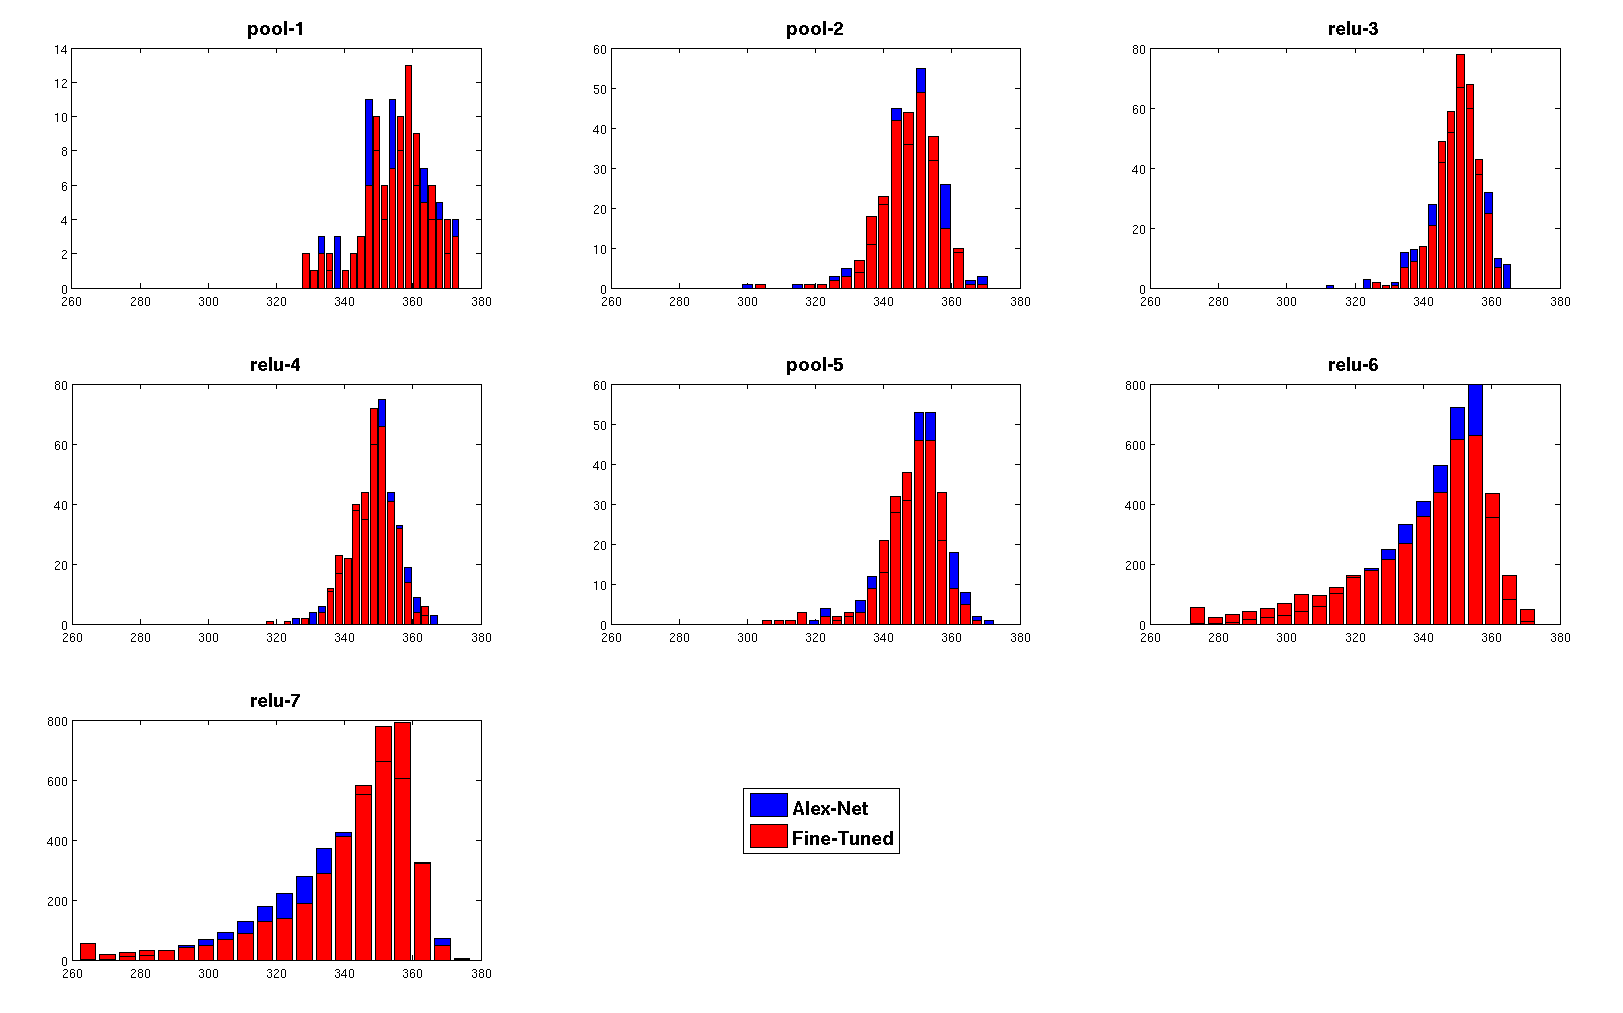
\includegraphics[height=6.5cm]{images/ent_hist.png}}
\caption{Distribution of AuE for different layers in Alex-Net and FT-Net. X-axis is the entropy and the Y-axis is the number of filters. Notice that the left tail for relu 6 and 7 becomes heavier after finetuning. This indicates that finetuning makes these filters more discriminative.}
\label{fig:fine-hist}
\end{figure}

\begin{figure}[t!]
\centering
\subfloat{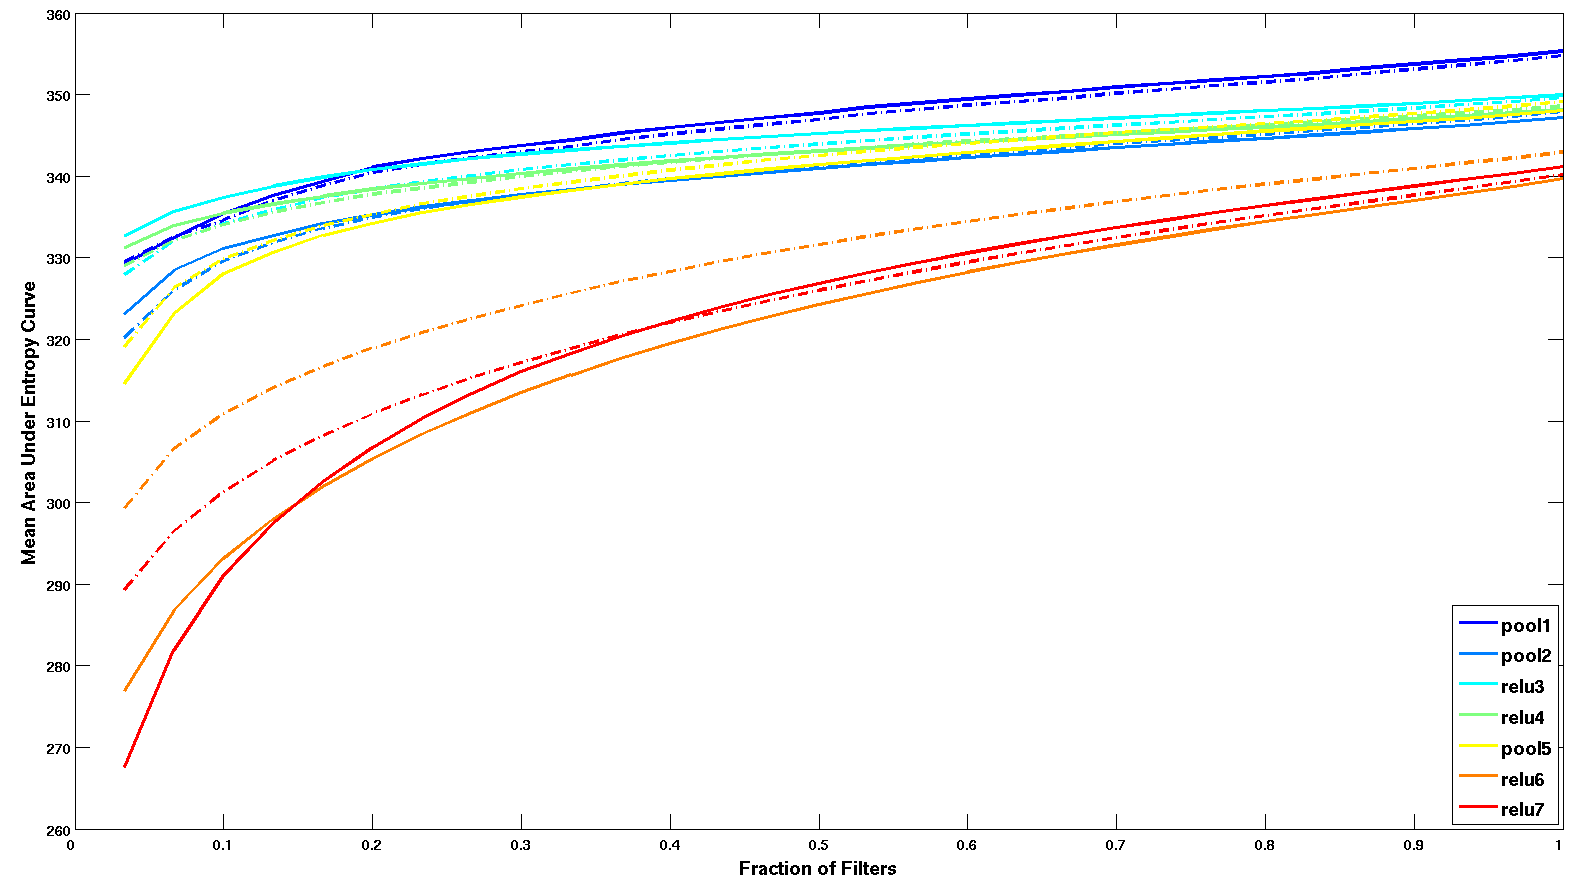
\includegraphics[scale=0.15]{images/entropy_variation.png}}
\caption{Mean Cumulative AuE plotted as fraction of filters (see sec \ref{sub:fine-entropy}). (Dash-Dot Line :Alex-Net, Solid Line: Fine-Tuned Network).}
\label{fig:fine-entropy}
\end{figure}

From figures \ref{fig:fine-hist} and \ref{fig:fine-entropy}, we draw 2 conclusions:
\begin{enumerate}
\item Although the entropy of filters decreases as we move to higher layers, the magnitude of change in entropy between layer 1 and layer 5 is small as compared to the change which happens when going from layer 5 to layer 6.
\item Finetuning mostly reduces the entropy of filters in the fully connected layers, there are small changes in layer 5 and negligible changes in other layers.
\end{enumerate} 
Table \ref{table:gt-bbox-fine} summarizes the classification mean AP obtained on classifying GT-BBOX  using features from different layers of a fine-tuned and a non-finetuned network.
\setlength{\tabcolsep}{4pt}
\begin{table}[t!]
\begin{center}
\caption{mAP for gt-bbox classification(FT: Fine-Tuned,A-Net: Alex-Net).}
\label{table:gt-bbox-fine}
\begin{tabular}{ccc|ccc|ccc|ccc}
\hline\noalign{\smallskip}
Layer & A-Net & FT & Layer & A-Net & FT & Layer & A-Net & FT & Layer & A-Net & FT \\
\noalign{\smallskip}
\hline
\noalign{\smallskip}
pool-1 & 43.2 & 43.2  & relu-3 & 73.3 & 73.7 & pool-5 & 79.1 & 82.2 & relu-7 & 84.0 & 87.1 \\
pool-2  & 67.1 & 67.7 & relu-4 & 75.5 & 77.8 & relu-6 & 83.4 & 85.4 \\
\hline
\end{tabular}
\end{center}
\end{table}
\setlength{\tabcolsep}{1.4pt}

\subsection{Is finetuning only the fully-connected layers sufficient?}
\label{sub:fine-fc-only}
The observations made in \ref{sub:fine-entropy} indicate that finetuning the convolutional layers in the CNN may not be critical for achieving good-performance on novel datasets. We test this hypothesis on the 2 challenging tasks of object detection(PASCAL) and scene classification (SUN-397) by comparing the performance of a fully finetuned network with a network finetuned by only updating weights in the fully-connected (fc) layers. Our results are summarized in table \ref{table:fine-effect}.

\setlength{\tabcolsep}{2pt}
\begin{table}[t!]
\begin{center}
\caption{Comparison in performance on of Alex-Net, Finetuned Network(ft-net) and a network with only fc layers finetuned (fc-ft).}
\label{table:fine-effect}
\scalebox{1}{
\begin{tabular}{|l|ccc|ccc|}
\hline
Layer & \multicolumn{3}{c}{detection(mAP)} & \multicolumn{3}{c|}{sun-397 (accuracy)} \\
\hline
      & alex-net & ft-net & fc-ft  & alex-net & ft-net & fc-ft\\
\hline
relu-7 & 45.5 & 54.1 & 53.3 & 53.1 & 56.1 & 55.5  \\
\hline
\end{tabular}}
\end{center}
\end{table}
\setlength{\tabcolsep}{1.4pt}

We find that indeed it is the case that the final performance in the detection setup only drops by 0.8 points and by 0.6 points for scene-classification. In our experiments we also noted accuracy of image classification on PASCAL is almost untouched by finetuning. This is suggestive of the fact finetuning is a task specific operation and finetuning for detection does not necessarily leads to an increase in classification performance, even though the classes and images are shared across PASCAL classification and detection challenges. 

\setlength{\tabcolsep}{1pt}
\begin{table}[t!]
\begin{center}
\caption{Evaluation of effect finetuning towards the task of object detection. (l5, l6, l7: layers 5, 6 and 7 of Alex Net)}
\label{table:det-fine}
\scalebox{0.75}{
\begin{tabular}{l|cccccccccccccccccccc||c}
\hline\noalign{\smallskip}
layer & aero & bike & bird & boat & bottle & bus & car & cat & chair & cow & table & dog & horse & mbike & person & plant & sheep & sofa & train & tv & mAP \\
\noalign{\smallskip}
\hline
l5 & 51.9 & 61.1 & 36.8 & 28.4 & 23.7 & 52.3 & 60.8 & 48.4 & 24.9 & 47.1 & 47.5 & 42.1 & 55.6 & 58.7 & 42.5 & 24.5 & 46.9 & 39.3 & 52.0 & 55.4 & 45.0 \\
l5-ft & 57.8 & 63.9 & 38.8 & 28.0 & 29.0&54.8&66.9&51.3 & 30.5 & 52.1 & 45.2 & 43.2 & 57.3 & 58.8 & 46.0 & 27.2 & 51.2 & 39.3 & 53.3 & 56.6 & 47.6 \\
\hline 
l6-ft &63.5 & 66.3 & 48.7 & 38.1 & 30.6 & 61.4 & 70.9 & 60.3 & 34.8 & 57.8 & 47.6 & 53.6 & 59.8 & 63.5 & 52.5 & 29.8 & 54.6 & 48.2 & 58.5 & 62.2 & 53.1 \\
l6-fc-ft& 61.4 & 63.9 & 44.2 & 36.2 & 29.0 & 59.9 & 66.0 & 55.3 & 31.1 & 57.6 & 49.5 & 49.4 & 59.4 & 63.7 & 50.8 & 29.5 & 54.1 & 43.2 & 57.4 & 58.8 & 51.0 \\
\hline
l7 & 57.6 & 57.2 & 41.4 & 31.2 & 25.6 & 52.4 & 58.8 & 50.9 & 25.2 & 50.4 & 42.7 & 47.1 & 52.2 & 55.6 & 44.5 & 23.9 & 48.0 & 38.1 & 51.5 & 56.6 & 45.5 \\
l7-ft & 64.3 & 69.6 & 50.1 & 41.8 & 32.0 & 62.6 & 71.0 & 60.6 & 32.8 & 58.5 & 46.4 & 56.0 & 60.0 & 66.9 & 54.2 & 31.5 & 52.7 & 48.8 & 57.7 & 64.7 & 54.1 \\
l7-fc-ft & 62.9 & 65.2 & 47.5 & 39.0 & 30.3 & 63.1 & 68.4 & 59.7 & 34.2 & 58.5 & 52.0 & 53.8 & 60.7 & 65.3 & 53.0 & 30.2 & 55.5 & 46.3 & 57.7 & 62.2 & 53.3 \\
\hline
\end{tabular}}
\end{center}
\end{table}
\setlength{\tabcolsep}{1.4pt}

A detailed layer-wise analysis of detection performance for all PASCAL classes and the 3 network configurations is presented in table \ref{table:det-fine}. Notice that for both the finetuned networks there is big jump in the performance while going from layer 5 to 6 and a rather small jump from layer 6 to 7. For Alex-Net, the performance is virtually the same for layers 5 and 7. It is also notable, that although the performance for FT-net is better by 2.6 points at layer 5 - the performance is virtually the same at layer 7. 
\subsection{Discussion}
\label{sub:fine-discussion}
Since layers 1-5 change a little over the course finetuning, this suggests that these are generic features. Although, one could always improve performance by a few points by finetuning the full network - for a lot of applications this may not be practical. 
It is also notable to point out that the more or less generic representations learnt in layer 4 and 5 are in contrast with some of the mid-level feature learning work such as \cite{Blocks} \cite{Mid1} wherein the problem of finding good mid-level parts is often posed as a greedy search for high recall discriminative templates.


\section{Is the information in the location or in the magnitude of filter activation?}
\label{sec-where-info}
Recent CNN based solutions for  classification, detection and localization ( \cite{overfeat}, \cite{Decaf},\cite{Rcnn}) have more or less treated CNN's as a black-box feature extractor. Such work has been limited to using either linear svm's, regression or a soft-max on top of vectorized layer features in contrast to the rich history of using structured multi-scale models in computer vision (\cite{DPM}, \cite{YangRamanan},\cite{Poselets}). In order to move away from black-box style of using CNN's and fully exploiting the potential which this feature hierarchy provides us with - it is instructive to tease apart what aspects of filter activation are important and what aspects can be ignored. 

In this work we focus on 2 particular questions:
\begin{itemize}
\item How important is the location where a filter fires?
\item How much information is contained in the magnitude of filter activations?
\end{itemize}

In order to answer these questions we constructed a series of ablation experiments (see fig \ref{fig:features}) and we use the difference in performance from the un-ablated feature representation (vectorized layer features) as a measure of how important each of these aspects is. We study these questions under the  settings of image classification (see table \ref{table:class-ablation}) and object detection using pool-5 features (see table\ref{table:det-ablation}). 

\begin{figure}[t!]
\centering
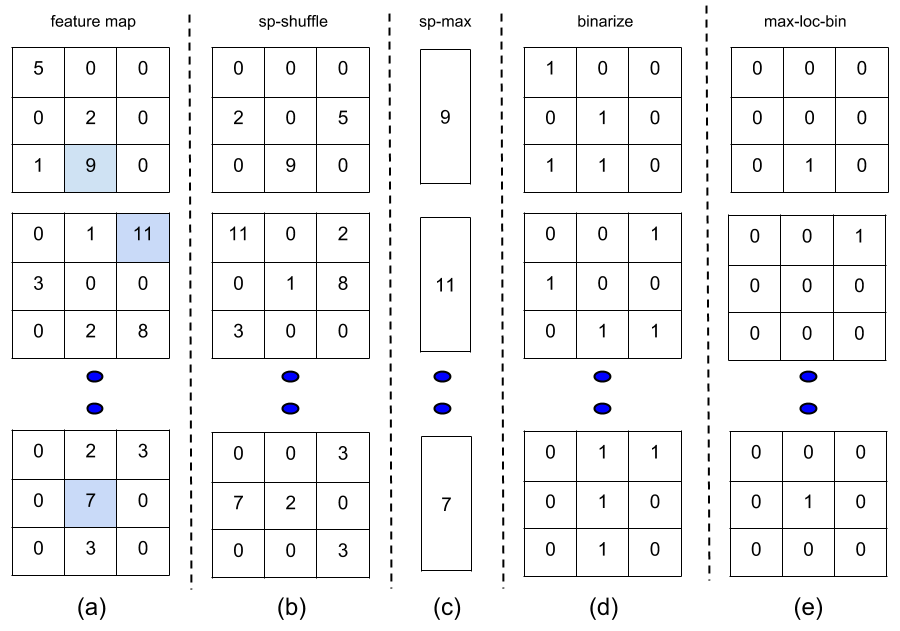
\includegraphics[height=6.5cm]{images/features1.png}
\caption{Description of feature ablations: For the purpose of illustration, consider each 3*3 block in (a) as the spatial activation of individual filters. Each block in (a) is a separate filter from the same layer. Ablation 1: \textit{spatial-shuffle-(b)} (sp-shuffle), involves applying an independent spatial random permutation to each feature map (different images see different permutations). Ablation 2: \textit{spatial max}-(c) (sp-max), select the max activation value in each feature map. Ablation 3: \textit{binarization}-(d) (bin). Ablation 4: \textit{sp-max-bin} - binarized sp-max.}
\label{fig:features}
\end{figure}

\subsection{How important is where a filter activates?}
\label{sub:imp-loc}
The two transformations which devoid the feature vector of any information about the location of where the filter activates (namely sp-max and sp-shuffle) seem to have a little effect on classification performance using pool-5 features. In contrast, for detection taking a spatial max (table \ref{table:det-ablation}) is disastrous and the performance drops by around 50\%. 
\setlength{\tabcolsep}{4pt}
\begin{table}[t!]
\begin{center}
\caption{Feature ablation analysis on PASCAL Image Classification (see fig \ref{fig:features})}
\label{table:class-ablation}
\begin{tabular}{lccccc}
\hline\noalign{\smallskip}
layer & unroll & sp-shuffle & sp-max & sp-max-bin & bin \\
\noalign{\smallskip}
\hline
\noalign{\smallskip}
pool-1 & 25.1 & 15.0 & 19.5 & 9.0 & 25.4  \\ 
pool-2 & 44.9 & 33.5 & 40.2 & - &43.0 \\ 
conv-3 & 50.1 & 40.4 & 54.2 & - &47.0 \\
conv-4 & 54.2 & 45.3 & 57.0 & - &51.3  \\
pool-5 & 65.6 & 59.6 & 62.6 & 27.2 &60.5 \\
relu-6 & 70.6 &  -   &  -   & -& 71.4     \\
relu-7 & 73.6 &  -   &  -   & - &74.1     \\
\hline
\end{tabular}
\end{center}
\end{table}
\setlength{\tabcolsep}{1.4pt}

\subsection{How important is the magnitude of activation ?}
\label{sub:imp-mag}
Binarization is the ablation which deprives features from their magnitude of activation. For classification, this results in a drop in performance greater than that due to sp-max. This suggests that it is more important to retain the magnitude than the location for classification. Rather, surprisingly binarization has little effect on detection performance.

\setlength{\tabcolsep}{1pt}
\begin{table}[t!]
\begin{center}
\caption{Effect of various feature ablations on object detection using R-CNN\cite{Rcnn}.}
\label{table:det-ablation}
\scalebox{0.70}{
\begin{tabular}{l|cccccccccccccccccccc||c}
\hline\noalign{\smallskip}
Feature & aero & bike & bird & boat & bottle & bus & car & cat & chair & cow & table & dog & horse & mbike & person & plant & sheep & sofa & train & tv & mAP \\
\noalign{\smallskip}
\hline
sp-max & 35.0 & 38.7 & 17.3 & 16.9 & 13.9 & 38.4 & 45.6 & 29.2 & 11.0 & 20.2 & 21.0 & 23.5 & 27.2 & 37.0 & 20.5 & 7.0 & 30.3 & 13.4 & 28.3 & 32.9 & 25.4 \\
bin & 57.9 & 61.3 & 32.6 & 24.7 & 27.5 & 55.0 & 64.7 & 49.8 & 25.3 & 47.4 & 44.5 & 40.3 & 54.6 & 56.4 & 43.6 & 27.1 & 48.4 & 41.6 & 54.3 & 57.6 & 45.7 \\
pool-5  & 57.8 & 63.9 & 38.8 & 28.0 & 29.0 & 54.8 & 66.9 & 51.3 & 30.5 & 52.1 & 45.2 & 43.2 & 57.3 & 58.8 & 46.0 & 27.2 & 51.2 & 39.3 & 53.3 & 56.6 & 47.6 \\
\noalign{\smallskip}
\hline
\end{tabular}}
\end{center}
\end{table}
\setlength{\tabcolsep}{1.4pt}



\subsection{Discussion}
Our experiments indicate that if the goal is classification layer 5 features can be treated as bag of filters without much loss in performance. We also find that different ablations effect different layers in different ways. For example, where as spatial-max is brutal for layer-1 it does not really effect classification is layer 5 features are used. On the other hand while binarization has little effect on layer-1 features it results into a drop of performance for layer-5. This is a good thing to know when designing systems which use features from multiple layers.

For classification although sp-max and binarization by themselves are not detrimental - their combination (sp-max-bin) is catastrophic to performance.

\section{Are there Grand-Mother Cells in CNN's? How distributed is the code?}
\label{sec:grand-mother}
How information is represented in deep architectures such as convolutional neural networks is an open question. We know that the first layer ends up learning gabor like edge detectors and that units in the final layers are very class specific. However, we are far from understanding the representations learned in the middle layers. Aprioiri it is unclear whether discriminative information about a certain class is encoded in distribution of a group of filter activations or whether there are specific units tuned to specific classes.

Some recent work such as \cite{DeConv}, \cite{Simonyan} have addressed this question by coming up with visualization techniques to understand tuning of various units. \cite{DeConv} present a deconvolution strategy for back-projecting into the image the regions which maximally activate a certain filter.  \cite{Simonyan}, on the other hand pose tuning as an optimization problem and try to estimate optimal stimuli for a given filter. \cite{GoogleCat} train a massive non-convolutional network and argue about the presence of cat and people specific filters in their network. Although visualizations are helpful, we feel they do not convey the full story. They are subjective and it is unclear what conclusions one might draw. In particular, visualizing the tuning of a few filters tells us very little about what the other filters might be doing. To best of our knowledge there is little work which tries to find an objective answer to this question.

Most of the above mentioned work can be mathematically treated either as estimating Prob(Filter Activity$\geq$ thresh $|$ Class) or finding the optimal stimulus for a specific unit. We argue that this by itself is an incomplete metric for interpreting how selective a certain filter is. (A hypothetical filter which has the same activation for all classes will score high on this measure.)  The right metric to evaluate if a certain filter is very selective (aka Grand-Mother Cell \cite{Barlow}) is precision defined as Prob(Class $|$Filter Activity $\geq$thresh)

We divide our analysis into two parts. In sec \ref{sub:class-specific-unit} we try to address if there exist filters with very high precision (aka Grand-Mother cells) and in sec \ref{sub:how-many} we answer how many filters are required to discriminate a class. 

\subsection{Are there high precision filters in layer 5?}
\label{sub:class-specific-unit}
Precision for each filter from layer 5 is computed in a way analogous to entropy computation described in \ref{sub:def-ent}. In the final step instead of computing the entropy, we compute Prob(Class $|$ Filter Activity $\geq$ threshold). We define the selectivity of a filter as the area under the precision curve. For this computation we use ground truth bounding boxes taken from PASCAL VOC-2007 test challenge.
From figure \ref{fig:prob-sel} it is clear that for some classes such persons and bicycles there are indeed some very high precision filters, but for a lot of classes like sofa and horses no such filters exist. 

\begin{figure}[t!]
\centering
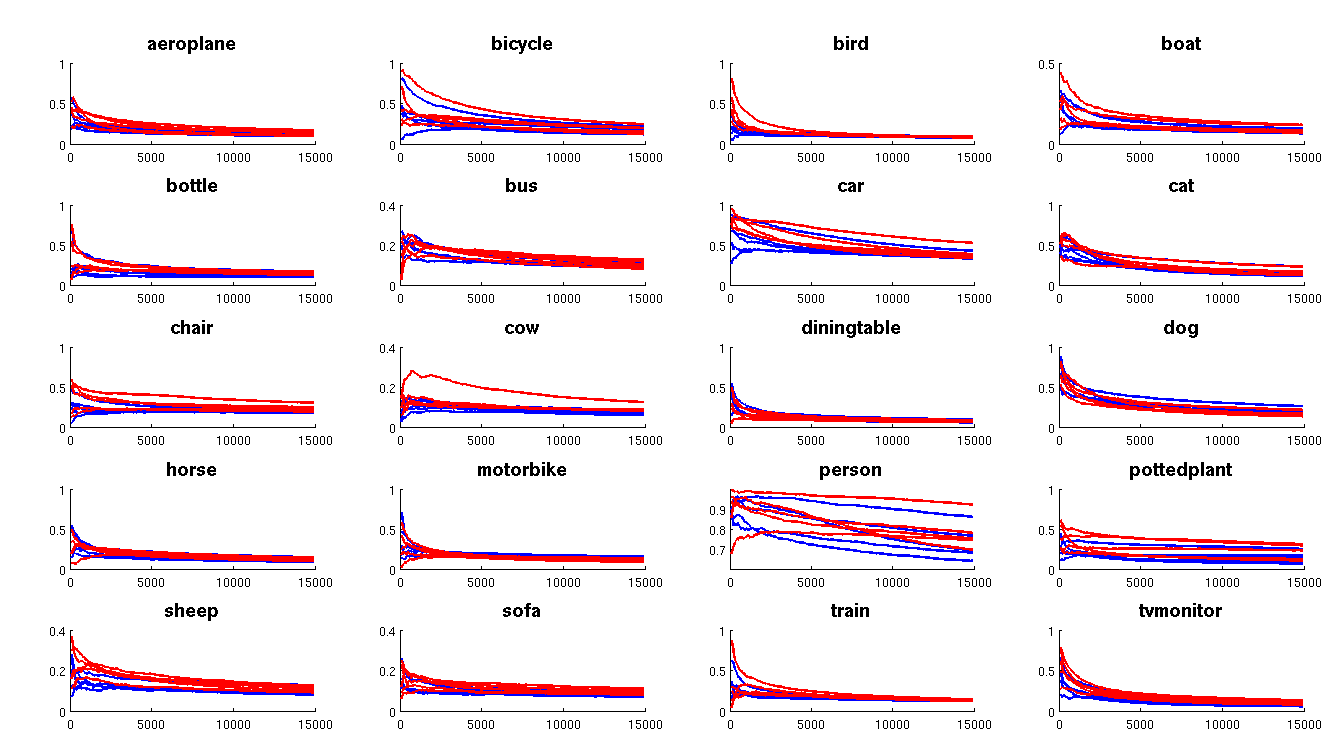
\includegraphics[scale=0.20]{images/prob_sel_dims_top5.png}
\caption{This plot shows the precision curve for the top 5 most selective filters taken from Alex-Net (Blue) and FT-Net(Red) for all PASCAL classes. Y-axis is the precision and X-axis is number of examples.}
\label{fig:prob-sel}
\end{figure}

\subsection{How many filters are required for discrimination?}
\label{sub:how-many}
In order to answer this question we train linear a svm for each class using only a subset of 256 pool-5 filters. In particular we construct subsets of size k, where k takes the values - [1,2,3,5,10,15,20,25,30,35,40,45, \newline 50,80, 100,128,256]. A subset of size k is constructed independently for each class using a greedy selection strategy described in figure \ref{fig:sel-strategy}. We use the variation in performance with the number of filters needed as a metric to evaluate how many filters are needed for each class. 
  
\begin{figure}[t!]
\centering
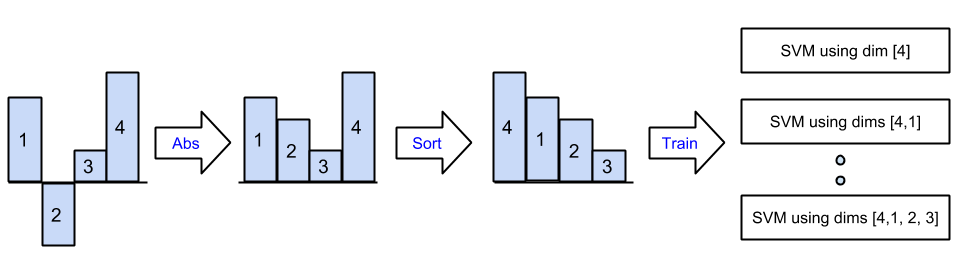
\includegraphics[scale=0.30]{images/how-many.png}
\caption{Illustration of our greedy strategy for constructing subsets of filters. For each class we first train a linear-svm using the spatial-max feature transformation described in section \ref{sub:imp-loc}. Spatial-max leaves us with a 256-D vector wherein each dimension has a one to one correspondence with 256 pool-5 filters. We use the magnitude of each dimension of the learnt weight vector as a proxy for the importance of that dimension towards discriminating a given class. For the purpose of illustration we describe the procedure with a 4-D weight vector shown on the extreme left (the numbers on each bar are the "dimension"). Firstly, we take the absolute value for each dimension and then sort the dimensions based on this value. Then, we chose the top k filters/dimensions from this ranked list to construct a subset of size k.}
\label{fig:sel-strategy}
\end{figure}

The results of our analysis are summarized in fig \ref{fig:svm-sel-dims} and table \ref{table:num-fil}. For classes such as persons, cars, cats we require a relatively few number of filters, but for most of the classes we need to look at around 30-40 filters to achieve atleast 90\% of the full performance. This also indicates, that for a few classes yes, there are grand-mother kind of neurons but for a lot of classes the representation is distributed. Also, as expected the fine-tuned network requires activations of a fewer numbers of filters to achieve the same performance but this reduction in number of filters is not large. 

\begin{figure}[t!]
\centering
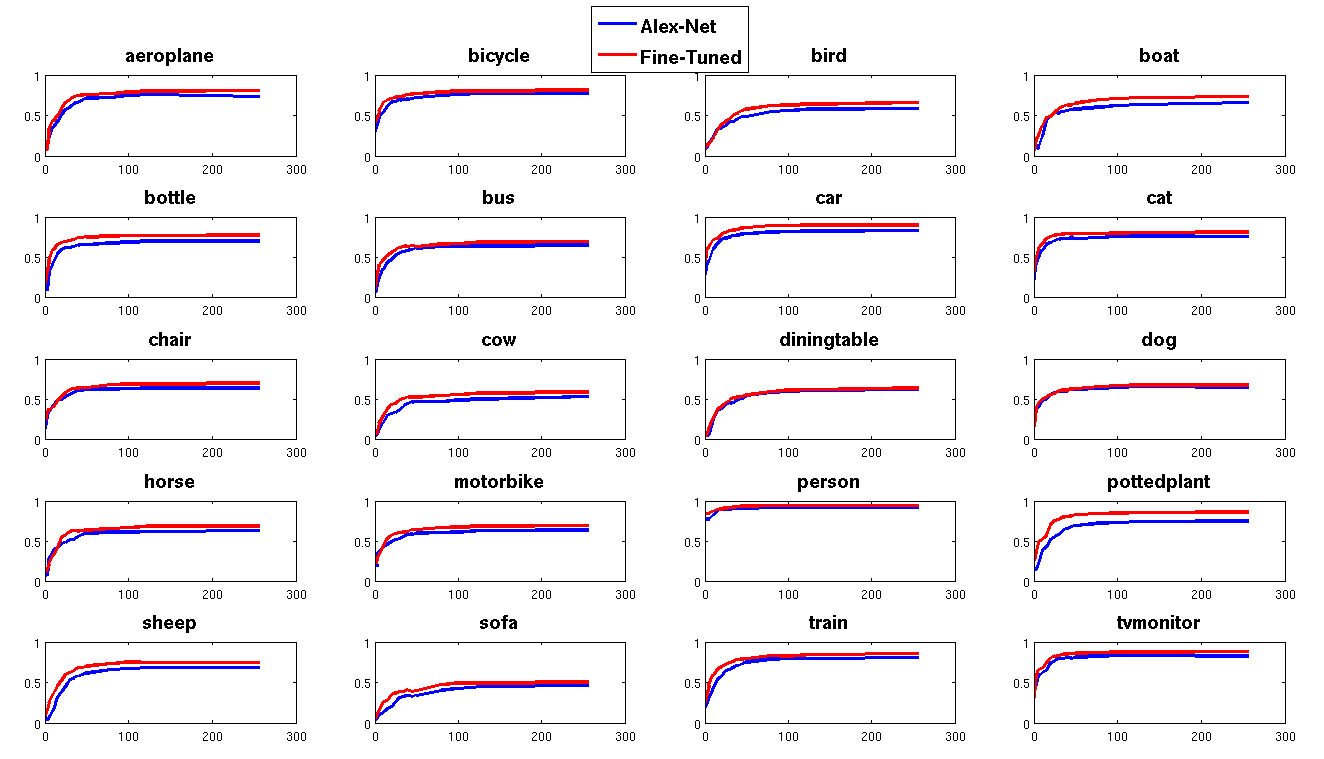
\includegraphics[height=6.5cm]{images/svm_seldims.png}
\caption{Analysis of how many filters are required to classify ground truth bounding boxes for 20 categories taken from PASCAL-2007 detection challenge. The y-axis in each of plot represents classification accuracy measured as mean-ap where as x-axis stand for the number of filters.)}
\label{fig:svm-sel-dims}
\end{figure}



\setlength{\tabcolsep}{1pt}
\begin{table}[t!]
\begin{center}
\caption{Number of filters required to achieve 50\% ,90\% of the full performance for PASCAL classes using Alex-Net(AN) and the Fine-Tuned network(FT)}
\label{table:num-fil}
\tiny
\begin{tabular}{lc||cccccccccccccccccccc}
\hline\noalign{\smallskip}
Net & AP & aero & bike & bird & boat & bottle & bus & car & cat & chair & cow & table & dog & horse & mbike & person & plant & sheep & sofa & train & tv \\
\noalign{\smallskip}
\hline
AN & 50 & 15 & 3 & 15 & 15 & 10 & 10 & 3 & 2 & 5 & 15 & 15 & 2 & 10 & 3 & 1 & 10 & 20 & 25 & 10 & 2 \\ 
FT & 50 & 10 & 1 & 20 & 15 & 5 & 5 & 2 & 2 & 3 & 10 & 15 & 3 & 15 & 10 & 1 & 5 & 15 & 15 & 5 & 2 \\
\hline
\noalign{\smallskip}
AN & 90 & 40 & 35 & 80 & 80 & 35 & 40 & 30 & 20 & 35 & 100 & 80 & 30 & 45 & 40 & 15 & 45 & 50 & 100 & 45 & 25 \\
FT & 90 & 35 & 30 & 80 & 80 & 30 & 35 & 25 & 20 & 35 & 50 & 80 & 35 & 30 & 40 & 10 & 35 & 40 & 80 & 40 & 20 \\
\hline
\end{tabular}
\end{center}
\end{table}
\setlength{\tabcolsep}{1.4pt}

\subsection{Discussion}
Although in our analysis we find that for discriminating some classes only a few units suffice whereas for others quite a lot of them are required. The ''extent" to which the code is distributed is likely to be a function of number of filters. If there are a few filters we will expect the code to be more distributed whereas if there are a large number of filters we expect to find more Grandmother kind of cells. The other important tradeoffs to consider are accuracy and training time as a function of number of filters in each layer. We as a community have only had a chance to experiment with a few network architectures out of the exponentially large number of possibilities. Although, it is beyond the scope of the current work determining the optimal number of filters in each layer is an open important question which needs to be addressed! 

\section{How do the different layers of a CNN train over time?}
\label{sec:speed}
Convolutional neural networks take a long time to train. For achieving state of art accuracy on the imagenet challenge these networks are often trained on high-end GPUs for more than 7 days. Even our implementation of fine-tuning following the approach proposed in \cite{Rcnn} takes more than 12 hours on a Nvidia Tesla-K40. Any speeds up in training will allow for a rich exploration of network architectures and parameters which is currently not possible.    

As a first step towards addressing this problem, we looked at the evolution of training loss and validation accuracy as the training progresses (fig \ref{fig:conv1}.) The top-1 accuracy on the imagenet validation set at 15K iterations is at 29.5 \% and 38.13\% at 50K iterations (compared to 57.4 \% at 310K iterations). The training loss rapidly increases initially and then there is a slow sluggish decay except at the stage where learning rate is decimated by a factor of 10 at 100K iterations.

\begin{figure}[t!]
\centering
\subfloat{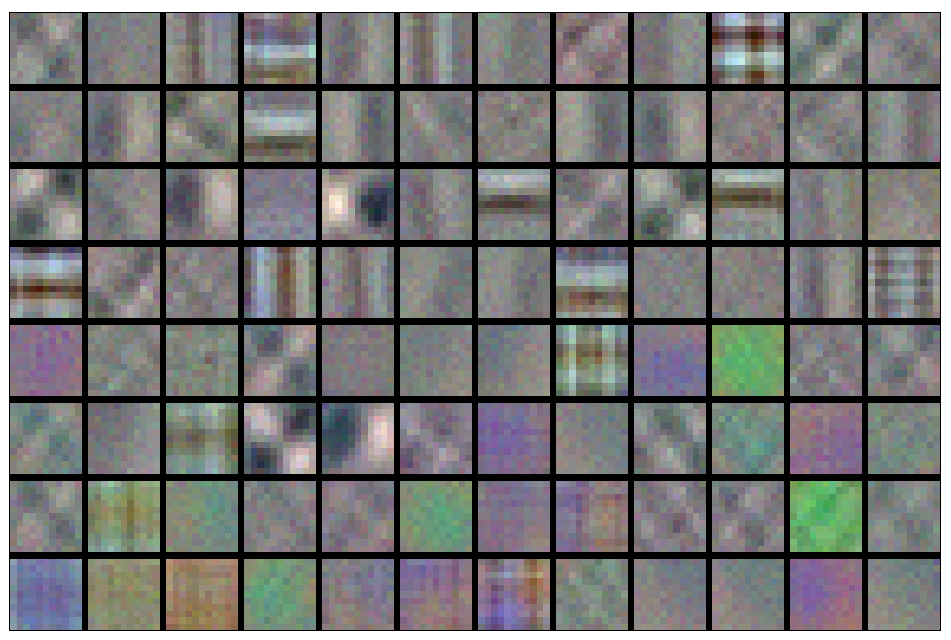
\includegraphics[scale=0.10]{images/l1_filters_iter5000.png}} \hspace{2mm}
\subfloat{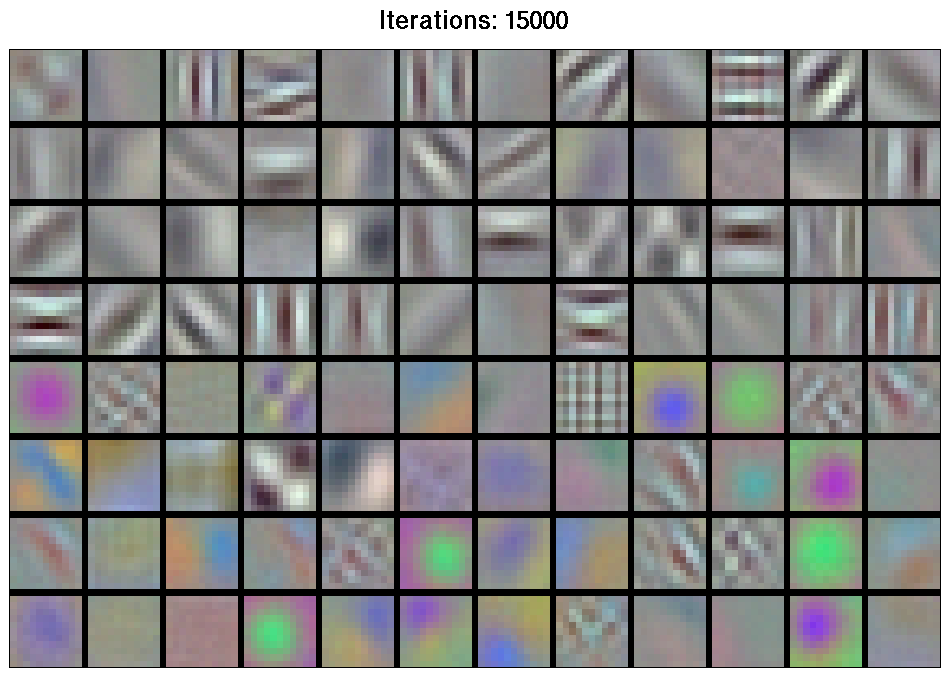
\includegraphics[scale=0.10]{images/l1_filters_iter15000.png}} \hspace{2mm}
\subfloat{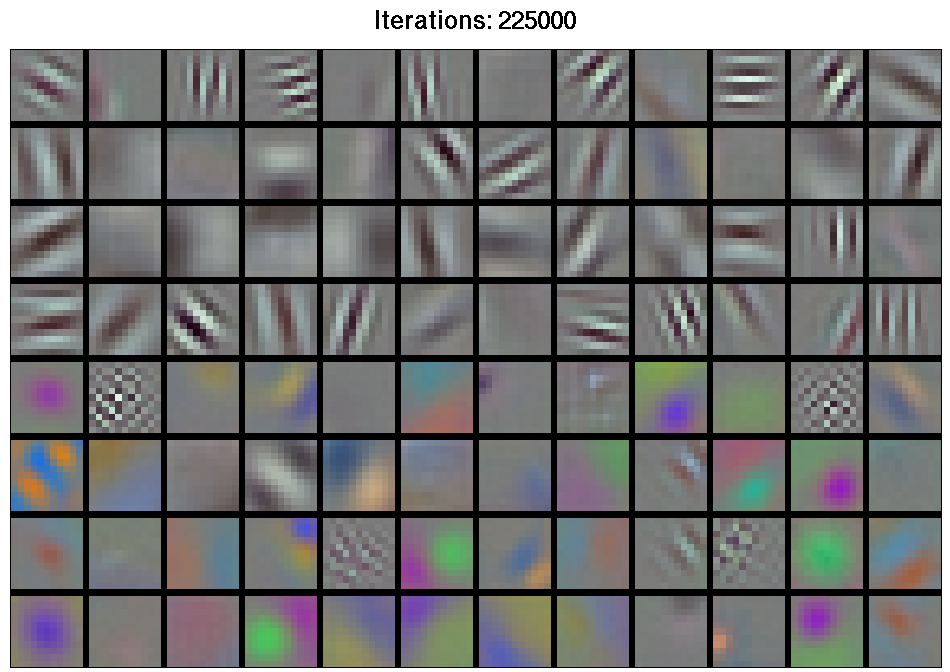
\includegraphics[scale=0.10]{images/l1_filters_iter225000.png}} \\
\subfloat{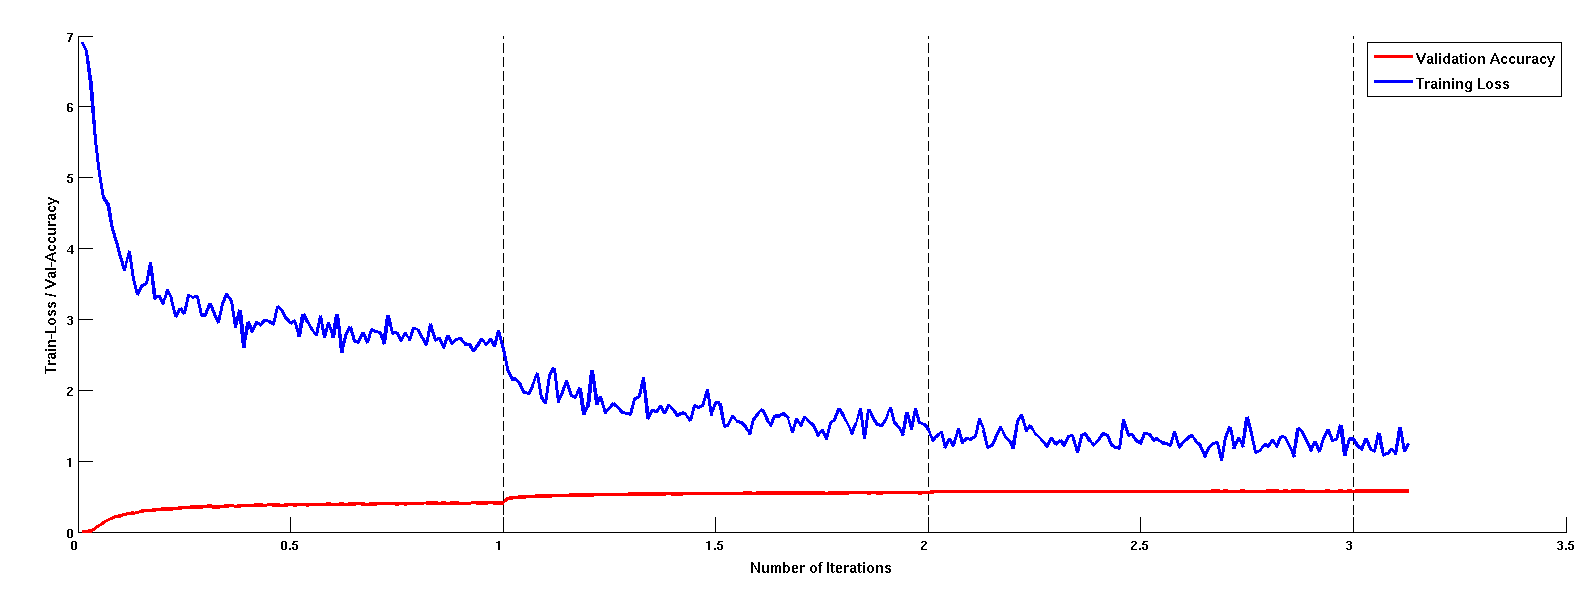
\includegraphics[scale=0.15]{images/training_loss.png}}
\caption{The first row shows conv-1 filters at 5K, 15K and 225K training iteration. The second row shows the evolution of training loss and top-1 accuracy on imagenet ilsvrc-2012 validation set as a function of number of iterations.}
\label{fig:conv1}
\end{figure}

The first question we ask is - Is there is an insightful interpretation of the fast initial drop in training loss? Towards this end, we visualized layer 1 filters at different time instances. Surprisingly, we found that within 15K iterations these filters look almost identical to what they would be by the end of the training (See fig \ref{fig:conv1}). This naturally leads us to ask the following questions: (a) How fast do different layers train? (b)Given that discriminative pre-training is helpful, is it the case that there exists a critical point after which learning on imagenet is not helpful for generalizing to other datasets/tasks? A ``yes" answer to this question would imply that we can indeed speed-up finetuning.


For a better understanding. we evaluated performance of a linear svm classifier learned on features extracted from individual layers on Pascal 2007 classification challenge. The results are summarized in table \ref{table:det-traj-classify}.It is quite surprising to note that by 15K iterations all layers are within 80\% and at 50K iterations within 90\% of there final performance. This strongly indicates that a great portion of training required for generalization happens quite quickly. 

\setlength{\tabcolsep}{4pt}
\begin{table}[t!]
\begin{center}
\caption{Variation in classification accuracy (mean-AP) on PASCAL VOC 2007 challenge using features extracted from different layers of Alex-Net as a function of number of iterations.}
\label{table:det-traj-classify}
\begin{tabular}{lcccccccc}
\hline\noalign{\smallskip}
Layer  & 5K & 15K & 25K & 35K & 45K & 95K & 105K & 310K \\
\noalign{\smallskip}
\hline
\noalign{\smallskip}
pool-1 & 23.0 & 24.3 & 24.4 & 24.5 & 24.6 & 24.8 & 24.7 & 25.1\\
pool-2 & 33.7 & 40.4 & 40.9 & 41.8 & 42.0 & 43.2 & 44.0 & 45.0\\
conv-3 & 34.2 & 46.8 & 47.0 & 48.2 & 48.5 & 49.4 & 51.6 & 50.1\\
conv-4 & 33.5 & 49.0 & 48.7 & 50.2 & 50.6 & 51.6 & 54.1 & 54.2\\
pool-5 & 33.0 & 53.4 & 55.0 & 56.8 & 57.4 & 59.2 & 63.5 & 65.6\\
relu-6 & 34.2 & 59.7 & 62.6 & 62.7 & 64.1 & 65.6 & 69.3 & 70.6\\
relu-7 & 30.9 & 61.3 & 64.1 & 65.1 & 65.8 & 67.8 & 71.8 & 73.2\\
\hline
\end{tabular}
\end{center}
\end{table}
\setlength{\tabcolsep}{1.4pt}

Motivated by these observations we trained a 50-50 network (50K iterations on imagenet and finetuned for 50K iterations using the procedure described in sec. \ref{sub:fine-train}) and evaluated its performance on the  Pascal 2007 detection challenge (see table \ref{table:det-trajectory} for results). Consistent with our earlier results we find that this network achieves a surprising performance of 48.6 mean AP points compared to 54.1 achieved by pre-training for 310K iterations. 

\setlength{\tabcolsep}{1pt}
\begin{table}[t!]
\begin{center}
\caption{Performance of 50-50 network for detection on pascal-voc-2007 challenge. (l5 is pool-5 and l7 is relu-7)}
\label{table:det-trajectory}
\scalebox{0.70}{
\begin{tabular}{l|cccccccccccccccccccc||c}
\hline\noalign{\smallskip}
Feature & aero & bike & bird & boat & bottle & bus & car & cat & chair & cow & table & dog & horse & mbike & person & plant & sheep & sofa & train & tv & mAP \\
\noalign{\smallskip}
\hline
l5(50-50) & 55.2 & 58.4 & 31.0 & 28.8 & 21.0 & 53.5 & 63.6 & 41.0 & 25.4 & 44.7 & 40.9 & 34.9 & 49.5 & 56.9 & 43.8 & 25.2 & 45.3 & 31.2 & 48.7 & 54.4 & 42.7 \\
l5 (full) & 57.8 & 63.9 & 38.8 & 28.0 & 29.0&54.8&66.9&51.3 & 30.5 & 52.1 & 45.2 & 43.2 & 57.3 & 58.8 & 46.0 & 27.2 & 51.2 & 39.3 & 53.3 & 56.6 & 47.6 \\
\hline
l7(50-50) & 58.7 & 64.8 & 38.2 & 34.9 & 25.9 & 59.5 & 69.5 & 46.2 & 28.7 & 52.4 & 45.2 & 44.3 & 57.3 & 63.4 & 52.4 & 28.0 & 51.5 & 34.9 & 56.0 & 59.4 & 48.6 \\
l7(full) & 64.3 & 69.6 & 50.1 & 41.8 & 32.0 & 62.6 & 71.0 & 60.6 & 32.8 & 58.5 & 46.4 & 56.0 & 60.0 & 66.9 & 54.2 & 31.5 & 52.7 & 48.8 & 57.7 & 64.7 & 54.1 \\
\hline
\end{tabular}}
\end{center}
\end{table}
\setlength{\tabcolsep}{1.4pt}
The above analysis reinforces our belief that indeed majority of training required for generalization happens quite quickly as compared to the full training time of the network. This observation suggest that there may exist clever ways which can help us speed up the training.
\section{Conclusion}
\label{sec:conclusion}
In this paper we analysed different properties of convolutional neural networks with the aim of gaining insights required to efficiently exploit the rich feature hierarchies provided by such networks.

\bibliographystyle{splncs}
\bibliography{egbib}
\end{document}
